\documentclass[twoside]{book}

% Packages required by doxygen
\usepackage{fixltx2e}
\usepackage{calc}
\usepackage{doxygen}
\usepackage[export]{adjustbox} % also loads graphicx
\usepackage{graphicx}
\usepackage[utf8]{inputenc}
\usepackage{makeidx}
\usepackage{multicol}
\usepackage{multirow}
\PassOptionsToPackage{warn}{textcomp}
\usepackage{textcomp}
\usepackage[nointegrals]{wasysym}
\usepackage[table]{xcolor}

% NLS support packages
\usepackage[spanish]{babel}
% Font selection
\usepackage[T1]{fontenc}
\usepackage[scaled=.90]{helvet}
\usepackage{courier}
\usepackage{amssymb}
\usepackage{sectsty}
\renewcommand{\familydefault}{\sfdefault}
\allsectionsfont{%
  \fontseries{bc}\selectfont%
  \color{darkgray}%
}
\renewcommand{\DoxyLabelFont}{%
  \fontseries{bc}\selectfont%
  \color{darkgray}%
}
\newcommand{\+}{\discretionary{\mbox{\scriptsize$\hookleftarrow$}}{}{}}

% Page & text layout
\usepackage{geometry}
\geometry{%
  a4paper,%
  top=2.5cm,%
  bottom=2.5cm,%
  left=2.5cm,%
  right=2.5cm%
}
\tolerance=750
\hfuzz=15pt
\hbadness=750
\setlength{\emergencystretch}{15pt}
\setlength{\parindent}{0cm}
\setlength{\parskip}{3ex plus 2ex minus 2ex}
\makeatletter
\renewcommand{\paragraph}{%
  \@startsection{paragraph}{4}{0ex}{-1.0ex}{1.0ex}{%
    \normalfont\normalsize\bfseries\SS@parafont%
  }%
}
\renewcommand{\subparagraph}{%
  \@startsection{subparagraph}{5}{0ex}{-1.0ex}{1.0ex}{%
    \normalfont\normalsize\bfseries\SS@subparafont%
  }%
}
\makeatother

% Headers & footers
\usepackage{fancyhdr}
\pagestyle{fancyplain}
\fancyhead[LE]{\fancyplain{}{\bfseries\thepage}}
\fancyhead[CE]{\fancyplain{}{}}
\fancyhead[RE]{\fancyplain{}{\bfseries\leftmark}}
\fancyhead[LO]{\fancyplain{}{\bfseries\rightmark}}
\fancyhead[CO]{\fancyplain{}{}}
\fancyhead[RO]{\fancyplain{}{\bfseries\thepage}}
\fancyfoot[LE]{\fancyplain{}{}}
\fancyfoot[CE]{\fancyplain{}{}}
\fancyfoot[RE]{\fancyplain{}{\bfseries\scriptsize Generado por Doxygen }}
\fancyfoot[LO]{\fancyplain{}{\bfseries\scriptsize Generado por Doxygen }}
\fancyfoot[CO]{\fancyplain{}{}}
\fancyfoot[RO]{\fancyplain{}{}}
\renewcommand{\footrulewidth}{0.4pt}
\renewcommand{\chaptermark}[1]{%
  \markboth{#1}{}%
}
\renewcommand{\sectionmark}[1]{%
  \markright{\thesection\ #1}%
}

% Indices & bibliography
\usepackage{natbib}
\usepackage[titles]{tocloft}
\setcounter{tocdepth}{3}
\setcounter{secnumdepth}{5}
\makeindex

% Hyperlinks (required, but should be loaded last)
\usepackage{ifpdf}
\ifpdf
  \usepackage[pdftex,pagebackref=true]{hyperref}
\else
  \usepackage[ps2pdf,pagebackref=true]{hyperref}
\fi
\hypersetup{%
  colorlinks=true,%
  linkcolor=blue,%
  citecolor=blue,%
  unicode%
}

% Custom commands
\newcommand{\clearemptydoublepage}{%
  \newpage{\pagestyle{empty}\cleardoublepage}%
}

\usepackage{caption}
\captionsetup{labelsep=space,justification=centering,font={bf},singlelinecheck=off,skip=4pt,position=top}

%===== C O N T E N T S =====

\begin{document}

% Titlepage & ToC
\hypersetup{pageanchor=false,
             bookmarksnumbered=true,
             pdfencoding=unicode
            }
\pagenumbering{alph}
\begin{titlepage}
\vspace*{7cm}
\begin{center}%
{\Large Netcp }\\
\vspace*{1cm}
{\large Generado por Doxygen 1.8.13}\\
\end{center}
\end{titlepage}
\clearemptydoublepage
\pagenumbering{roman}
\tableofcontents
\clearemptydoublepage
\pagenumbering{arabic}
\hypersetup{pageanchor=true}

%--- Begin generated contents ---
\chapter{netcp}
\label{md_README}
\Hypertarget{md_README}
Netcp es la implementación de un programa cliente-\/servidor utilizado para la transferencia de ficheros múltiple y simultánea.

Hace uso de\+: -\/\+Sockets en linux -\/\+Hilos en C++ ($<$thread$>$) 
\chapter{Indice jerárquico}
\section{Jerarquía de la clase}
Esta lista de herencias esta ordenada aproximadamente por orden alfabético\+:\begin{DoxyCompactList}
\item \contentsline{section}{Message}{\pageref{structMessage}}{}
\item \contentsline{section}{received\+\_\+info}{\pageref{structreceived__info}}{}
\item \contentsline{section}{server}{\pageref{classserver}}{}
\item \contentsline{section}{Socket\+\_\+base}{\pageref{classSocket__base}}{}
\begin{DoxyCompactList}
\item \contentsline{section}{Socket\+\_\+af}{\pageref{classSocket__af}}{}
\begin{DoxyCompactList}
\item \contentsline{section}{Socket\+\_\+af\+\_\+dgram}{\pageref{classSocket__af__dgram}}{}
\end{DoxyCompactList}
\end{DoxyCompactList}
\end{DoxyCompactList}

\chapter{Índice de clases}
\section{Lista de clases}
Lista de las clases, estructuras, uniones e interfaces con una breve descripción\+:\begin{DoxyCompactList}
\item\contentsline{section}{\hyperlink{structMessage}{Message} \\*Representa un mensaje P\+OD (Plain old data) con un texto de 1024 bytes (caracteres) }{\pageref{structMessage}}{}
\item\contentsline{section}{\hyperlink{structreceived__info}{received\+\_\+info} \\*Envuelve una sockaddr\+\_\+in con la información del Socket que ha enviado el mensaje y un booleano para saber si se ha recibido un mensaje }{\pageref{structreceived__info}}{}
\item\contentsline{section}{\hyperlink{classserver}{server} \\*Implementa el servidor netcp }{\pageref{classserver}}{}
\item\contentsline{section}{\hyperlink{classSocket__af}{Socket\+\_\+af} \\*Clase abstracta de un socket perteneciente a la familia A\+F\+\_\+\+I\+N\+ET Es decir, que permite \char`\"{}conexiones\char`\"{} tanto desde el mismo equipo como desde equipos externos }{\pageref{classSocket__af}}{}
\item\contentsline{section}{\hyperlink{classSocket__af__dgram}{Socket\+\_\+af\+\_\+dgram} \\*Socket de la familia A\+F\+\_\+\+I\+N\+ET y no orientado a conexión }{\pageref{classSocket__af__dgram}}{}
\item\contentsline{section}{\hyperlink{classSocket__base}{Socket\+\_\+base} \\*Clase abstracta base para un socket }{\pageref{classSocket__base}}{}
\end{DoxyCompactList}

\chapter{Indice de archivos}
\section{Lista de archivos}
Lista de todos los archivos documentados y con descripciones breves\+:\begin{DoxyCompactList}
\item\contentsline{section}{/home/alejandro/\+Documentos/github\+\_\+me/netcp/include/{\bfseries client.\+hpp} }{\pageref{client_8hpp}}{}
\item\contentsline{section}{/home/alejandro/\+Documentos/github\+\_\+me/netcp/include/{\bfseries Message.\+hpp} }{\pageref{Message_8hpp}}{}
\item\contentsline{section}{/home/alejandro/\+Documentos/github\+\_\+me/netcp/include/{\bfseries received\+\_\+info.\+hpp} }{\pageref{received__info_8hpp}}{}
\item\contentsline{section}{/home/alejandro/\+Documentos/github\+\_\+me/netcp/include/{\bfseries server.\+hpp} }{\pageref{server_8hpp}}{}
\item\contentsline{section}{/home/alejandro/\+Documentos/github\+\_\+me/netcp/include/{\bfseries Socket\+\_\+af.\+hpp} }{\pageref{Socket__af_8hpp}}{}
\item\contentsline{section}{/home/alejandro/\+Documentos/github\+\_\+me/netcp/include/{\bfseries Socket\+\_\+af\+\_\+dgram.\+hpp} }{\pageref{Socket__af__dgram_8hpp}}{}
\item\contentsline{section}{/home/alejandro/\+Documentos/github\+\_\+me/netcp/include/\hyperlink{Socket__base_8hpp}{Socket\+\_\+base.\+hpp} \\*Clase abstracta Socket }{\pageref{Socket__base_8hpp}}{}
\item\contentsline{section}{/home/alejandro/\+Documentos/github\+\_\+me/netcp/include/{\bfseries transf\+\_\+info.\+hpp} }{\pageref{transf__info_8hpp}}{}
\end{DoxyCompactList}

\chapter{Documentación de las clases}
\hypertarget{structMessage}{}\section{Referencia de la Estructura Message}
\label{structMessage}\index{Message@{Message}}


Representa un mensaje P\+OD (Plain old data) con un texto de 1024 bytes (caracteres)  




{\ttfamily \#include $<$Message.\+hpp$>$}

\subsection*{Atributos públicos}
\begin{DoxyCompactItemize}
\item 
\mbox{\Hypertarget{structMessage_a8398aec0171dec03c496704e79fd0022}\label{structMessage_a8398aec0171dec03c496704e79fd0022}} 
std\+::array$<$ char, 1024 $>$ {\bfseries text}
\item 
\mbox{\Hypertarget{structMessage_aaeff602e34763cb97a9fe25d435f7164}\label{structMessage_aaeff602e34763cb97a9fe25d435f7164}} 
int {\bfseries code\+\_\+}
\item 
\mbox{\Hypertarget{structMessage_af6c004d9113d8d6590cc717ebe4a8c48}\label{structMessage_af6c004d9113d8d6590cc717ebe4a8c48}} 
int {\bfseries port\+\_\+}
\end{DoxyCompactItemize}


\subsection{Descripción detallada}
Representa un mensaje P\+OD (Plain old data) con un texto de 1024 bytes (caracteres) 

Codes\+: 0 -\/ 1 -\/ 2 -\/ 3 -\/ Continuar envío al puerto indicado en port\+\_\+ 

La documentación para esta estructura fue generada a partir del siguiente fichero\+:\begin{DoxyCompactItemize}
\item 
/home/alejandro/\+Documentos/github\+\_\+me/netcp/include/Message.\+hpp\end{DoxyCompactItemize}

\hypertarget{classSocket}{}\section{Referencia de la Clase Socket}
\label{classSocket}\index{Socket@{Socket}}


\subsection{Descripción detallada}
familia A\+F\+\_\+\+I\+N\+ET y no orientado a conexión 

La documentación para esta clase fue generada a partir del siguiente fichero\+:\begin{DoxyCompactItemize}
\item 
/home/alejandro/\+Documentos/github\+\_\+me/netcp/include/Socket\+\_\+af\+\_\+dgram.\+hpp\end{DoxyCompactItemize}

\hypertarget{classSocket__af}{}\section{Referencia de la Clase Socket\+\_\+af}
\label{classSocket__af}\index{Socket\+\_\+af@{Socket\+\_\+af}}


Clase abstracta de un socket perteneciente a la familia A\+F\+\_\+\+I\+N\+ET Es decir, que permite \char`\"{}conexiones\char`\"{} tanto desde el mismo equipo como desde equipos externos.  




{\ttfamily \#include $<$Socket\+\_\+af.\+hpp$>$}



Diagrama de herencias de Socket\+\_\+af
\nopagebreak
\begin{figure}[H]
\begin{center}
\leavevmode
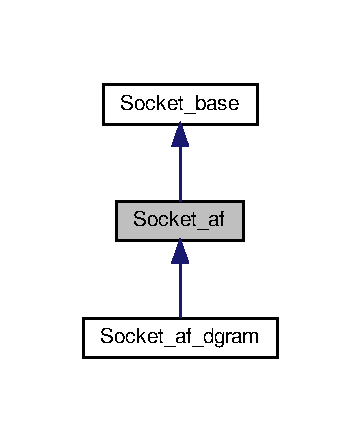
\includegraphics[width=173pt]{classSocket__af__inherit__graph}
\end{center}
\end{figure}


Diagrama de colaboración para Socket\+\_\+af\+:\nopagebreak
\begin{figure}[H]
\begin{center}
\leavevmode
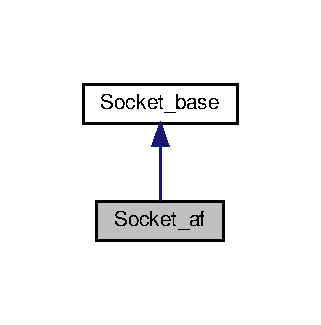
\includegraphics[width=154pt]{classSocket__af__coll__graph}
\end{center}
\end{figure}
\subsection*{Métodos públicos}
\begin{DoxyCompactItemize}
\item 
sockaddr\+\_\+in \hyperlink{classSocket__af_aa2f8fb1398c1e6f66832151e8c5bcf2e}{get\+\_\+sockaddr\+\_\+in\+\_\+from} (const std\+::string ip\+\_\+address, int \hyperlink{classSocket__base_afcdd7ae81a9fb867d012b7db8c259576}{port})
\begin{DoxyCompactList}\small\item\em Devuelve sockaddr\+\_\+in inicializada. \end{DoxyCompactList}\end{DoxyCompactItemize}


\subsection{Descripción detallada}
Clase abstracta de un socket perteneciente a la familia A\+F\+\_\+\+I\+N\+ET Es decir, que permite \char`\"{}conexiones\char`\"{} tanto desde el mismo equipo como desde equipos externos. 

\begin{DoxyAuthor}{Autor}
Miguel Martín 
\end{DoxyAuthor}
\begin{DoxyDate}{Fecha}
20200919 
\end{DoxyDate}


\subsection{Documentación de las funciones miembro}
\mbox{\Hypertarget{classSocket__af_aa2f8fb1398c1e6f66832151e8c5bcf2e}\label{classSocket__af_aa2f8fb1398c1e6f66832151e8c5bcf2e}} 
\index{Socket\+\_\+af@{Socket\+\_\+af}!get\+\_\+sockaddr\+\_\+in\+\_\+from@{get\+\_\+sockaddr\+\_\+in\+\_\+from}}
\index{get\+\_\+sockaddr\+\_\+in\+\_\+from@{get\+\_\+sockaddr\+\_\+in\+\_\+from}!Socket\+\_\+af@{Socket\+\_\+af}}
\subsubsection{\texorpdfstring{get\+\_\+sockaddr\+\_\+in\+\_\+from()}{get\_sockaddr\_in\_from()}}
{\footnotesize\ttfamily sockaddr\+\_\+in Socket\+\_\+af\+::get\+\_\+sockaddr\+\_\+in\+\_\+from (\begin{DoxyParamCaption}\item[{const std\+::string}]{ip\+\_\+address,  }\item[{int}]{port }\end{DoxyParamCaption})\hspace{0.3cm}{\ttfamily [virtual]}}



Devuelve sockaddr\+\_\+in inicializada. 


\begin{DoxyParams}{Parámetros}
{\em ip\+\_\+address} & Dirección ip a bindear al socket \\
\hline
{\em port} & Puerto a bindear al socket \\
\hline
\end{DoxyParams}


Implementa \hyperlink{classSocket__base_a887249ae6a25693230c0febf403a2545}{Socket\+\_\+base}.



La documentación para esta clase fue generada a partir de los siguientes ficheros\+:\begin{DoxyCompactItemize}
\item 
/home/alejandro/\+Documentos/github\+\_\+me/netcp/include/Socket\+\_\+af.\+hpp\item 
/home/alejandro/\+Documentos/github\+\_\+me/netcp/src/Socket\+\_\+af.\+cpp\end{DoxyCompactItemize}

\hypertarget{classSocket__af__dgram}{}\section{Referencia de la Clase Socket\+\_\+af\+\_\+dgram}
\label{classSocket__af__dgram}\index{Socket\+\_\+af\+\_\+dgram@{Socket\+\_\+af\+\_\+dgram}}


{\ttfamily \#include $<$Socket\+\_\+af\+\_\+dgram.\+hpp$>$}



Diagrama de herencias de Socket\+\_\+af\+\_\+dgram\nopagebreak
\begin{figure}[H]
\begin{center}
\leavevmode
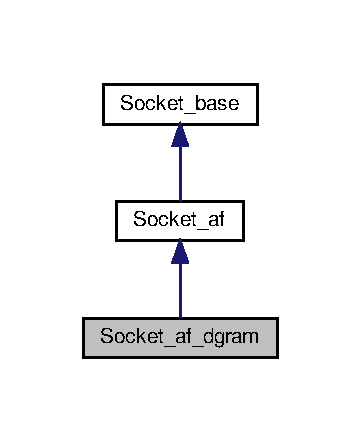
\includegraphics[width=173pt]{classSocket__af__dgram__inherit__graph}
\end{center}
\end{figure}


Diagrama de colaboración para Socket\+\_\+af\+\_\+dgram\+:\nopagebreak
\begin{figure}[H]
\begin{center}
\leavevmode
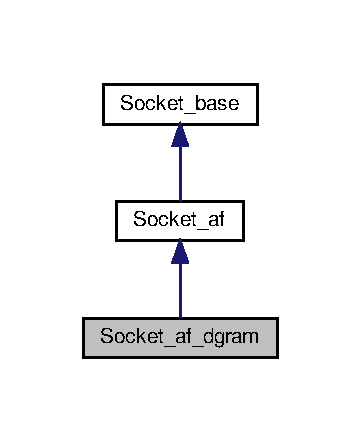
\includegraphics[width=173pt]{classSocket__af__dgram__coll__graph}
\end{center}
\end{figure}
\subsection*{Métodos públicos}
\begin{DoxyCompactItemize}
\item 
\hyperlink{classSocket__af__dgram_a11391f68bb56dafa6be879f388e4b0cd}{Socket\+\_\+af\+\_\+dgram} (std\+::string \hyperlink{classSocket__base_aed490170422026c6dfe5def12031cd04}{ip}, int \hyperlink{classSocket__base_afcdd7ae81a9fb867d012b7db8c259576}{port})
\item 
void \hyperlink{classSocket__af__dgram_a6a2084d50ab117b0bf6b699aa0573db5}{bindsock} (int \hyperlink{classSocket__base_a740aedbac3269e4981732dd6842cd9c2}{fd}, std\+::string \hyperlink{classSocket__base_aed490170422026c6dfe5def12031cd04}{ip}, int \hyperlink{classSocket__base_afcdd7ae81a9fb867d012b7db8c259576}{port})
\begin{DoxyCompactList}\small\item\em Bindea el socket a la ip y puerto especificados. \end{DoxyCompactList}\item 
void \hyperlink{classSocket__af__dgram_a744bb661eeebe5b5cdfca0028da6bd88}{send\+\_\+to} (\hyperlink{structMessage}{Message} msg, std\+::string remote\+\_\+ip, int remote\+\_\+port)
\begin{DoxyCompactList}\small\item\em Envía el mensaje {\itshape msg} al socket bindeado a la dirección {\itshape remote\+\_\+ip} y puerto {\itshape remote\+\_\+port}. \end{DoxyCompactList}\item 
sockaddr\+\_\+in \hyperlink{classSocket__af__dgram_a572c1e9c58c11512fa75d0ad7a775857}{receive} (\hyperlink{structMessage}{Message} $\ast$msg)
\begin{DoxyCompactList}\small\item\em Recive un mensaje y lo guarda en el \hyperlink{structMessage}{Message} apuntado por {\itshape msg}. \end{DoxyCompactList}\end{DoxyCompactItemize}


\subsection{Descripción detallada}
\begin{DoxyAuthor}{Autor}
Miguel Martín 
\end{DoxyAuthor}
\begin{DoxyDate}{Fecha}
20200919 
\end{DoxyDate}


\subsection{Documentación del constructor y destructor}
\mbox{\Hypertarget{classSocket__af__dgram_a11391f68bb56dafa6be879f388e4b0cd}\label{classSocket__af__dgram_a11391f68bb56dafa6be879f388e4b0cd}} 
\index{Socket\+\_\+af\+\_\+dgram@{Socket\+\_\+af\+\_\+dgram}!Socket\+\_\+af\+\_\+dgram@{Socket\+\_\+af\+\_\+dgram}}
\index{Socket\+\_\+af\+\_\+dgram@{Socket\+\_\+af\+\_\+dgram}!Socket\+\_\+af\+\_\+dgram@{Socket\+\_\+af\+\_\+dgram}}
\subsubsection{\texorpdfstring{Socket\+\_\+af\+\_\+dgram()}{Socket\_af\_dgram()}}
{\footnotesize\ttfamily Socket\+\_\+af\+\_\+dgram\+::\+Socket\+\_\+af\+\_\+dgram (\begin{DoxyParamCaption}\item[{std\+::string}]{ip,  }\item[{int}]{port }\end{DoxyParamCaption})}

\begin{DoxyAuthor}{Autor}
Miguel Martín 
\end{DoxyAuthor}
\begin{DoxyDate}{Fecha}
20200919 
\end{DoxyDate}


\subsection{Documentación de las funciones miembro}
\mbox{\Hypertarget{classSocket__af__dgram_a6a2084d50ab117b0bf6b699aa0573db5}\label{classSocket__af__dgram_a6a2084d50ab117b0bf6b699aa0573db5}} 
\index{Socket\+\_\+af\+\_\+dgram@{Socket\+\_\+af\+\_\+dgram}!bindsock@{bindsock}}
\index{bindsock@{bindsock}!Socket\+\_\+af\+\_\+dgram@{Socket\+\_\+af\+\_\+dgram}}
\subsubsection{\texorpdfstring{bindsock()}{bindsock()}}
{\footnotesize\ttfamily void Socket\+\_\+af\+\_\+dgram\+::bindsock (\begin{DoxyParamCaption}\item[{int}]{fd,  }\item[{std\+::string}]{ip,  }\item[{int}]{port }\end{DoxyParamCaption})}



Bindea el socket a la ip y puerto especificados. 


\begin{DoxyParams}{Parámetros}
{\em ip} & Dirección ip a la que bindear el socket \\
\hline
{\em port} & Puerto al que bindear el socket \\
\hline
\end{DoxyParams}
\mbox{\Hypertarget{classSocket__af__dgram_a572c1e9c58c11512fa75d0ad7a775857}\label{classSocket__af__dgram_a572c1e9c58c11512fa75d0ad7a775857}} 
\index{Socket\+\_\+af\+\_\+dgram@{Socket\+\_\+af\+\_\+dgram}!receive@{receive}}
\index{receive@{receive}!Socket\+\_\+af\+\_\+dgram@{Socket\+\_\+af\+\_\+dgram}}
\subsubsection{\texorpdfstring{receive()}{receive()}}
{\footnotesize\ttfamily sockaddr\+\_\+in Socket\+\_\+af\+\_\+dgram\+::receive (\begin{DoxyParamCaption}\item[{\hyperlink{structMessage}{Message} $\ast$}]{msg }\end{DoxyParamCaption})}



Recive un mensaje y lo guarda en el \hyperlink{structMessage}{Message} apuntado por {\itshape msg}. 


\begin{DoxyParams}{Parámetros}
{\em msg} & Puntero a una estructura {\itshape \hyperlink{structMessage}{Message}} \\
\hline
\end{DoxyParams}
\begin{DoxyReturn}{Devuelve}
Retorna una struct sockaddr\+\_\+in con la dirección de donde ha recibido el mensaje 
\end{DoxyReturn}
\mbox{\Hypertarget{classSocket__af__dgram_a744bb661eeebe5b5cdfca0028da6bd88}\label{classSocket__af__dgram_a744bb661eeebe5b5cdfca0028da6bd88}} 
\index{Socket\+\_\+af\+\_\+dgram@{Socket\+\_\+af\+\_\+dgram}!send\+\_\+to@{send\+\_\+to}}
\index{send\+\_\+to@{send\+\_\+to}!Socket\+\_\+af\+\_\+dgram@{Socket\+\_\+af\+\_\+dgram}}
\subsubsection{\texorpdfstring{send\+\_\+to()}{send\_to()}}
{\footnotesize\ttfamily void Socket\+\_\+af\+\_\+dgram\+::send\+\_\+to (\begin{DoxyParamCaption}\item[{\hyperlink{structMessage}{Message}}]{msg,  }\item[{std\+::string}]{remote\+\_\+ip,  }\item[{int}]{remote\+\_\+port }\end{DoxyParamCaption})}



Envía el mensaje {\itshape msg} al socket bindeado a la dirección {\itshape remote\+\_\+ip} y puerto {\itshape remote\+\_\+port}. 


\begin{DoxyParams}{Parámetros}
{\em remote\+\_\+ip} & Dirección ip remota \\
\hline
{\em remote\+\_\+port} & Puerto remoto \\
\hline
\end{DoxyParams}


La documentación para esta clase fue generada a partir de los siguientes ficheros\+:\begin{DoxyCompactItemize}
\item 
include/hierarchy/Socket\+\_\+af\+\_\+dgram.\+hpp\item 
src/hierarchy/Socket\+\_\+af\+\_\+dgram.\+cpp\end{DoxyCompactItemize}

\hypertarget{classSocket__base}{}\section{Referencia de la Clase Socket\+\_\+base}
\label{classSocket__base}\index{Socket\+\_\+base@{Socket\+\_\+base}}


Clase abstracta base para un socket.  




{\ttfamily \#include $<$Socket\+\_\+base.\+hpp$>$}



Diagrama de herencias de Socket\+\_\+base\nopagebreak
\begin{figure}[H]
\begin{center}
\leavevmode
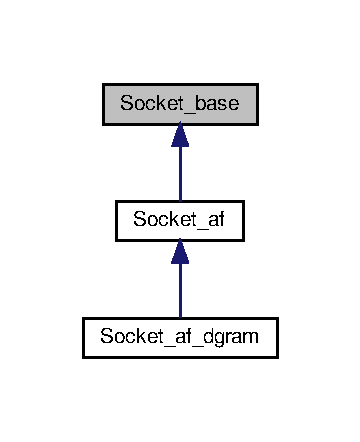
\includegraphics[width=173pt]{classSocket__base__inherit__graph}
\end{center}
\end{figure}
\subsection*{Métodos públicos}
\begin{DoxyCompactItemize}
\item 
std\+::string \hyperlink{classSocket__base_aed490170422026c6dfe5def12031cd04}{ip} (void)
\begin{DoxyCompactList}\small\item\em Devuelve la ip del socket. \end{DoxyCompactList}\item 
\mbox{\Hypertarget{classSocket__base_ad70da7f9fc273f0f2fa847447c292038}\label{classSocket__base_ad70da7f9fc273f0f2fa847447c292038}} 
void \hyperlink{classSocket__base_ad70da7f9fc273f0f2fa847447c292038}{set\+\_\+fd} (int \hyperlink{classSocket__base_a740aedbac3269e4981732dd6842cd9c2}{fd})
\begin{DoxyCompactList}\small\item\em Settea el fd y verifica errores. \end{DoxyCompactList}\item 
int \hyperlink{classSocket__base_afcdd7ae81a9fb867d012b7db8c259576}{port} (void)
\begin{DoxyCompactList}\small\item\em Devuelve el puerto del socket. \end{DoxyCompactList}\item 
\mbox{\Hypertarget{classSocket__base_a740aedbac3269e4981732dd6842cd9c2}\label{classSocket__base_a740aedbac3269e4981732dd6842cd9c2}} 
int \hyperlink{classSocket__base_a740aedbac3269e4981732dd6842cd9c2}{fd} (void)
\begin{DoxyCompactList}\small\item\em Devuelve el descriptor de fichero del socket. \end{DoxyCompactList}\item 
void \hyperlink{classSocket__base_af0b9f713f4d6231c287198034fad662e}{initialize} (void)
\begin{DoxyCompactList}\small\item\em Inicializa ip\+\_\+ y port\+\_\+ una vez bindeado el socket. \end{DoxyCompactList}\item 
virtual sockaddr\+\_\+in \hyperlink{classSocket__base_a887249ae6a25693230c0febf403a2545}{get\+\_\+sockaddr\+\_\+in\+\_\+from} (const std\+::string ip\+\_\+address, int \hyperlink{classSocket__base_afcdd7ae81a9fb867d012b7db8c259576}{port})=0
\begin{DoxyCompactList}\small\item\em Devuelve sockaddr\+\_\+in inicializada. \end{DoxyCompactList}\end{DoxyCompactItemize}


\subsection{Descripción detallada}
Clase abstracta base para un socket. 

\subsection{Documentación de las funciones miembro}
\mbox{\Hypertarget{classSocket__base_a887249ae6a25693230c0febf403a2545}\label{classSocket__base_a887249ae6a25693230c0febf403a2545}} 
\index{Socket\+\_\+base@{Socket\+\_\+base}!get\+\_\+sockaddr\+\_\+in\+\_\+from@{get\+\_\+sockaddr\+\_\+in\+\_\+from}}
\index{get\+\_\+sockaddr\+\_\+in\+\_\+from@{get\+\_\+sockaddr\+\_\+in\+\_\+from}!Socket\+\_\+base@{Socket\+\_\+base}}
\subsubsection{\texorpdfstring{get\+\_\+sockaddr\+\_\+in\+\_\+from()}{get\_sockaddr\_in\_from()}}
{\footnotesize\ttfamily virtual sockaddr\+\_\+in Socket\+\_\+base\+::get\+\_\+sockaddr\+\_\+in\+\_\+from (\begin{DoxyParamCaption}\item[{const std\+::string}]{ip\+\_\+address,  }\item[{int}]{port }\end{DoxyParamCaption})\hspace{0.3cm}{\ttfamily [pure virtual]}}



Devuelve sockaddr\+\_\+in inicializada. 


\begin{DoxyParams}{Parámetros}
{\em ip\+\_\+address} & Dirección ip a bindear al socket \\
\hline
{\em port} & Puerto a bindear al socket \\
\hline
\end{DoxyParams}


Implementado en \hyperlink{classSocket__af_aa2f8fb1398c1e6f66832151e8c5bcf2e}{Socket\+\_\+af}.

\mbox{\Hypertarget{classSocket__base_af0b9f713f4d6231c287198034fad662e}\label{classSocket__base_af0b9f713f4d6231c287198034fad662e}} 
\index{Socket\+\_\+base@{Socket\+\_\+base}!initialize@{initialize}}
\index{initialize@{initialize}!Socket\+\_\+base@{Socket\+\_\+base}}
\subsubsection{\texorpdfstring{initialize()}{initialize()}}
{\footnotesize\ttfamily void Socket\+\_\+base\+::initialize (\begin{DoxyParamCaption}\item[{void}]{ }\end{DoxyParamCaption})}



Inicializa ip\+\_\+ y port\+\_\+ una vez bindeado el socket. 

Es necesario que el socket ya esté bindeado, dado que esta función hace uso de getsockname() para conocer la ip y el puerto. \mbox{\Hypertarget{classSocket__base_aed490170422026c6dfe5def12031cd04}\label{classSocket__base_aed490170422026c6dfe5def12031cd04}} 
\index{Socket\+\_\+base@{Socket\+\_\+base}!ip@{ip}}
\index{ip@{ip}!Socket\+\_\+base@{Socket\+\_\+base}}
\subsubsection{\texorpdfstring{ip()}{ip()}}
{\footnotesize\ttfamily std\+::string Socket\+\_\+base\+::ip (\begin{DoxyParamCaption}\item[{void}]{ }\end{DoxyParamCaption})}



Devuelve la ip del socket. 

\begin{DoxyReturn}{Devuelve}
Objeto std\+::string que es la dirección ip a la que el socket está bindeado. 
\end{DoxyReturn}
\mbox{\Hypertarget{classSocket__base_afcdd7ae81a9fb867d012b7db8c259576}\label{classSocket__base_afcdd7ae81a9fb867d012b7db8c259576}} 
\index{Socket\+\_\+base@{Socket\+\_\+base}!port@{port}}
\index{port@{port}!Socket\+\_\+base@{Socket\+\_\+base}}
\subsubsection{\texorpdfstring{port()}{port()}}
{\footnotesize\ttfamily int Socket\+\_\+base\+::port (\begin{DoxyParamCaption}\item[{void}]{ }\end{DoxyParamCaption})}



Devuelve el puerto del socket. 

\begin{DoxyReturn}{Devuelve}
int que es el puerto al que el socket está bindeado. 
\end{DoxyReturn}


La documentación para esta clase fue generada a partir de los siguientes ficheros\+:\begin{DoxyCompactItemize}
\item 
include/hierarchy/\hyperlink{Socket__base_8hpp}{Socket\+\_\+base.\+hpp}\item 
src/hierarchy/Socket\+\_\+base.\+cpp\end{DoxyCompactItemize}

\chapter{Documentación de archivos}
\hypertarget{Socket__base_8hpp}{}\section{Referencia del Archivo include/hierarchy/\+Socket\+\_\+base.hpp}
\label{Socket__base_8hpp}\index{include/hierarchy/\+Socket\+\_\+base.\+hpp@{include/hierarchy/\+Socket\+\_\+base.\+hpp}}


Clase abstracta \hyperlink{classSocket}{Socket}.  


{\ttfamily \#include $<$array$>$}\newline
{\ttfamily \#include $<$netinet/in.\+h$>$}\newline
{\ttfamily \#include $<$string$>$}\newline
Dependencia gráfica adjunta para Socket\+\_\+base.\+hpp\+:\nopagebreak
\begin{figure}[H]
\begin{center}
\leavevmode
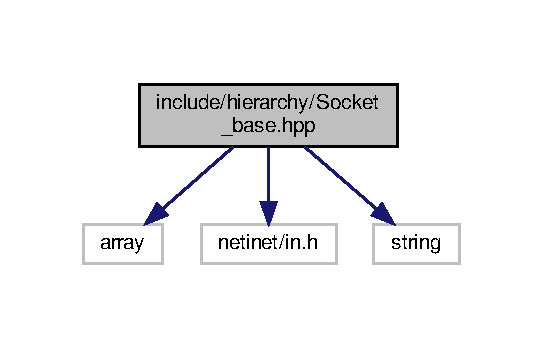
\includegraphics[width=261pt]{Socket__base_8hpp__incl}
\end{center}
\end{figure}
Gráfico de los archivos que directa o indirectamente incluyen a este archivo\+:\nopagebreak
\begin{figure}[H]
\begin{center}
\leavevmode
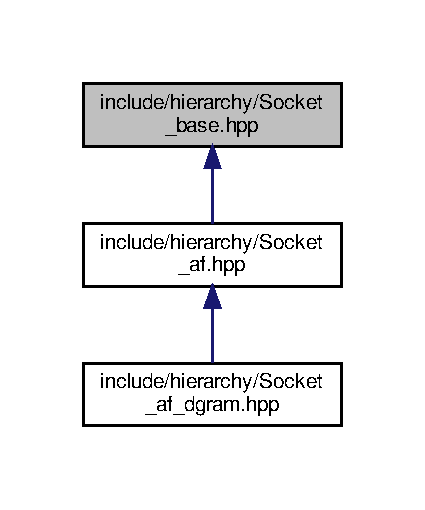
\includegraphics[width=204pt]{Socket__base_8hpp__dep__incl}
\end{center}
\end{figure}
\subsection*{Clases}
\begin{DoxyCompactItemize}
\item 
struct \hyperlink{structMessage}{Message}
\begin{DoxyCompactList}\small\item\em Representa un mensaje P\+OD (Plain old data) con un texto de 1024 bytes (caracteres) \end{DoxyCompactList}\item 
class \hyperlink{classSocket__base}{Socket\+\_\+base}
\begin{DoxyCompactList}\small\item\em Clase abstracta base para un socket. \end{DoxyCompactList}\end{DoxyCompactItemize}


\subsection{Descripción detallada}
Clase abstracta \hyperlink{classSocket}{Socket}. 

\begin{DoxyAuthor}{Autor}
Miguel Martín 
\end{DoxyAuthor}
\begin{DoxyDate}{Fecha}
20200919 
\end{DoxyDate}

%--- End generated contents ---

% Index
\backmatter
\newpage
\phantomsection
\clearemptydoublepage
\addcontentsline{toc}{chapter}{Índice}
\printindex

\end{document}
